\label{subseq:mumps-review}

Originally, \acrfull{mumps} was a part of the PARASOL Project. The project was an ESPRIT IV long term research with the main goal to build and test a portable library for solving large sparse systems of equations on distributed memory systems \cite{PARASOL}. An important aspect of the research was a strong link between the developers of the sparse solvers and industrial end users, who provided a range of test problems and evaluated the solvers \cite{MUMPS:description}. Since 2000, \acrshort{mumps} had continued as an ongoing project and the library have contained almost 5 main releases, at the moment of writing.\\



As it was mentioned in Section \ref{subseq:mm-library-choice}, \acrshort{mumps} is an implementation of the multifrontal method. Therefore, \acrshort{mumps} performs all three phases in sequence, namely: analysis, numerical factorization and solution. The numerical factorization and solution phases were fully described in detail in Subsection \ref{subseq:direct-sparse methods}. In this section, the analysis phase of \acrshort{mumps} is examined since implementations of this phase often vary between libraries due to different  performance considerations.\\


According to the library documentation, the analysis phases of \acrshort{mumps} consists of several pre-processing steps:

\begin{enumerate}
  \item Fill reducing reordering \label{mumps:analysis-steps:1}
  \item Symbolic factorization \label{mumps:analysis-steps:2}
  \item Scaling \label{mumps:analysis-steps:3}
  \item Amalgamantion \label{mumps:analysis-steps:4}
  \item Mapping \label{mumps:analysis-steps:5}
\end{enumerate}


% Fill-reducing pivot order
\ref{mumps:analysis-steps:1}) To handle both symmetric and unsymmetric cases, \acrshort{mumps} performs fill reducing reordering based on $\boldsymbol{A} + \boldsymbol{A^T}$ sparsity pattern. The library provides numerous sequantial algorithms for the reordering such as Approximate Minimum Degree (AMD) \cite{reordering:AMD}, Approximate Minimum Fill (AMF), Approximate Minimum Degree with automatic quasi-dense row detection (QAMD) \cite{reordering:QAMD}, Bottom-up and Top-down Sparse Reordering (PORD) \cite{reordering:PORD}, Nested Dissection coupled with AMD (Scotch) \cite{reordering:SCOTCH}, Multilevel Nested Dissection coupled with Multiple Minimum Degree (METIS) \cite{reordering:METIS}. Additionally, \acrshort{mumps} can work together with ParMETIS and PT-Scotch which are extensions of METIS and Scotch libraries for parallel execution, respectively. \acrshort{mumps} also provides users with an option to select a fill-in reducing algorithm in run-time based on a matrix type, size and the number of processors \cite{mumps-manual}.\\


% Symbolic factorization
\ref{mumps:analysis-steps:2}) Sparsity structures of factors $L$ and $U$ are computed during the symbolic factorization pre-processing step, based on permuted matrix $A$ after fill-in reducing reordering. It gives the input information for the elimination tree building process.  All computations are performed using an undirected graph $G(A)$ associated with a matrix $A$ at this step.\\


% Scaling
%\ref{mumps:analysis-steps:3}) Matrix $A$ is tried to be scaled in such a way to get absolute values of \textit{one} along the main diagonal and \textit{less than one} for all off-diagonal entries. 


\ref{mumps:analysis-steps:3}) Rows and/or columns of matrix $A$ can be scaled during either the analysis or factorization phase in order to improve numerical solution accuracy. As an additional consequence, this pre-processing step can result in more reliable estimations of required memory space and load balancing, performed during the analysis phase, due to a reduced amount of pivoting during numerical factorization. Different scaling approaches are adopted in MUMPS, namely: diagonal, column or column-row scalings during the numerical factorization phase, see \cite{mumps-manual} for details; scalings based on works \cite{mm:scaling:duff1999design}, \cite{mm:scaling:duff2001algorithms} and \cite{mm:scaling:duff2005strategies} for the analysis phase.\\


%algorithms are described in detail in works \cite{mm:scaling:duff1999design}, \cite{mm:scaling:duff2001algorithms} (for  unsymmetric cases) and \cite{mm:scaling:duff2005strategies} (for  symmetric cases). This pre-processing step is supposed to improve numerical accuracy and make all estimations performed during the analysis phase more reliable \cite{mumps-manual}. \acrshort{mumps} also provides an option to switch off scaling or perform it during the factorization phase.\\



% Amalgamantion
\ref{mumps:analysis-steps:4}) During the  amalgamation step, described in Subsection \ref{subseq:direct-sparse methods}, sets of columns with the same off-diagonal sparsity pattern are group together to create denser nodes, also known as super-nodes. The process leads to restructuring the original elimination tree to an amalgamated one of super-nodes which is also know as the \textit{assembly tree}. The main purpose of this step is to improve efficiency of dense matrix operations.\\



% Mapping
%\ref{mumps:analysis-steps:5}) A host process, chosen by \acrshort{mumps}, creates a pool of tasks where each task  belongs to one out of three different types, Figure \ref{fig:mumps:mapping-and-scheduling}. Then, the host distributes tasks among all available processes in such a way to achieve good memory and compute balances.\\

\ref{mumps:analysis-steps:5}) A host process, chosen by \acrshort{mumps}, creates a pool of tasks where each task refers to partial factorization of a node i.e. a frontal matrix. Each node belongs to one of three different types according to a size of the frontal matrix that a node refers to. Type 1 and 2 nodes represent small- and medium-sized frontal matrices, respectively. Whereas a type 3 node  represents the root node of an assembly tree i.e the largest frontal matrix. \acrshort{mumps} uses different parallel computational strategies, that are explained below, in order to process nodes of different types with the aim of achieving better parallel performance. The host process distributes tasks among all available processes in such a way to achieve good memory and compute balances. Figure \ref{fig:mumps:mapping-and-scheduling} shows an example of a process distribution in \acrshort{mumps}.\\


Type 1 nodes are grouped in subtrees, according to the Geist-Ng algorithm \cite{geist1989task}, and each subtree is processed by a single process to avoid the finest task granularity, which can cause high communication overheads. \\


In case of type 2 nodes, the host process assigns each node to one process, called the \textit{master}, which holds fully summed rows and columns of a node as well as performs threshold pivoting and partial factorization. During the numerical factorization phase, in run-time, a master process first receives symbolic information, describing  contribution block structures, from its children. Then, the master collects information concerning the load balances of all other processes and decides, \underline{\textit{dynamically}},  which of them, \textit{slaves}, are going to participate in the node factorization. After that, the master informs the chosen slaves that a new task has been allocated for them; maps them according to a 1D block column distribution and sends them the corresponding parts of the frontal matrix. Then, the slaves communicate with  the children of the master process and collect the corresponding numerical values. The slaves are in charge of assembly and computations of the partly summed rows. The computational process is illustrated in Figure \ref{fig:mumps:steps-of-type-2-factorization}, Subsection \ref{subseq:blas-comparison}.\\


The root node belongs to the 3rd type. The host \underline{\textit{statically}} assigns a master for the root, as it is in case of type 2 nodes, to hold all the indices describing the structure of its frontal matrix. Before factorization, the structure of the root frontal matrix is statically mapped onto a 2D grid of processes using a block cyclic distribution. This allows to determine, during the analysis phase, which process an entry of the root is assigned to. Hence, the original matrix entries and parts of the contribution blocks can be assembled as soon as they are available. Because of threshold pivoting, the master process collects indices for all delayed variables of its sons; builds the final structure of the root frontal matrix and broadcasts the corresponding symbolic information to all slaves. The slaves, in turn, adjust their local data structure and, right after this, perform numerical factorization in parallel.\\


It is important to mention that if the root node size is less than a certain computer depended parameter value, defined internally by \acrshort{mumps}, the root node will be treated as a type 2 one, \cite{mumps-manual}.\\


An example of static/dynamic scheduling i.e. process mapping, is depicted in Figure \ref{fig:mumps:mapping-and-scheduling}.\\


\figpointer{\ref{fig:mumps:mapping-and-scheduling}}
\begin{figure}[htpb]
  \centering
  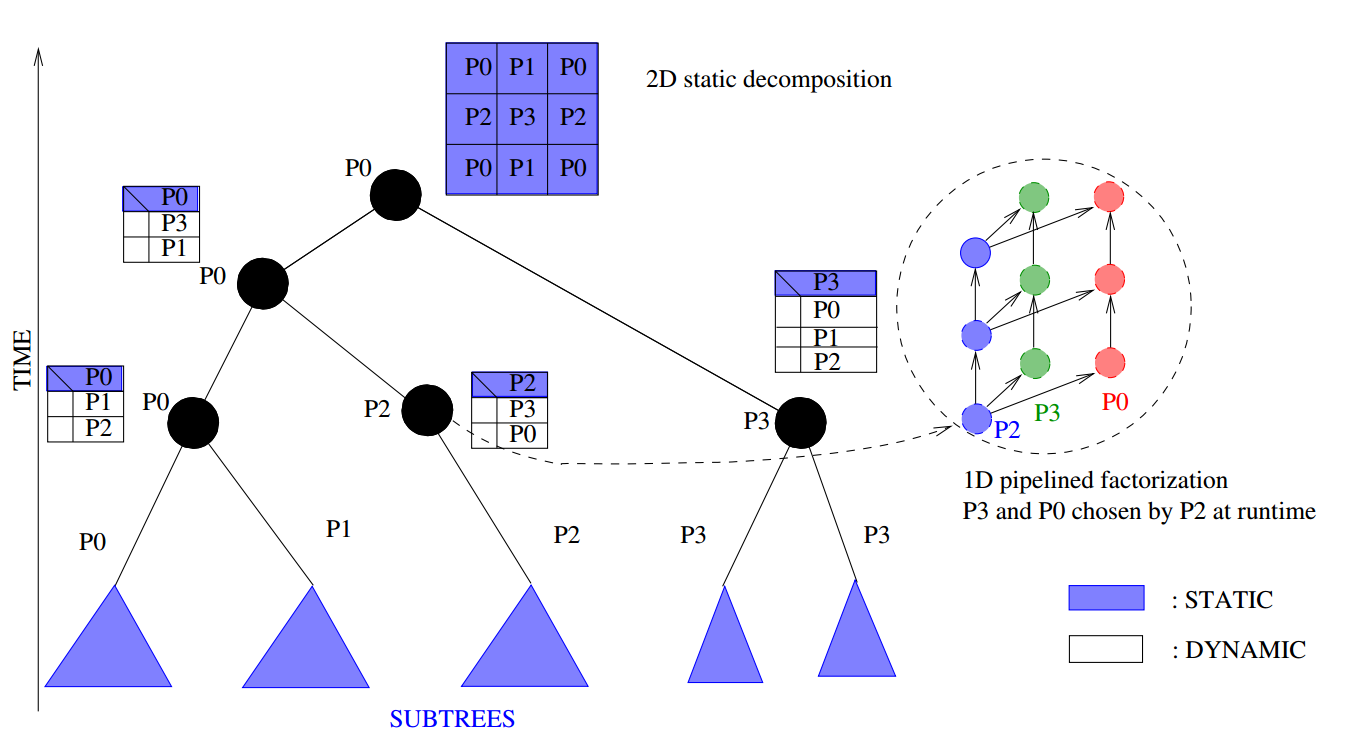
\includegraphics[width=0.85\textwidth]{figures/chapter-2/mumps-task-data-parallelism-2.png}
    \caption[An example of static and dynamic scheduling in \acrshort{mumps}]{An example of static and dynamic scheduling in \acrshort{mumps}, \cite{l2012multifrontal}}
\label{fig:mumps:mapping-and-scheduling}
\end{figure}


